\documentclass{article}
\title{Eletrostatics}
\author{Serafí Nebot Ginard}
\date{2022-2023}

\usepackage[parfill]{parskip}
\usepackage{amsmath}
\usepackage{tikz}

\begin{document}
\maketitle
\newpage

\tableofcontents
\newpage

\section{Punctual loads}

If we place a punctual load in space it will create an electric field towards all
surrounding points in space. Therefore, any point in space will have an associated vector $\vec{E}$
describing the magnitude and direction of the electric field produced by the puntual load
\[
	\vec{E} = \frac{1}{4\pi \epsilon_0}\frac{q}{r^2}r
\]
where $\epsilon_0$ is the vacuum permittivity, $q$ the punctual load, $r$ the distance between the
punctual load and the reference point, and $\hat{r}$ a unit vector indicating the direction
of the electric field towards the reference point.

Vectors of an electric field produced by a \emph{positive} punctual load will point outwards. Vectors of an electric field produced by a \emph{negative} punctual load will point inwards.

\begin{figure}[h]
	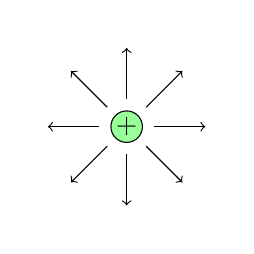
\begin{tikzpicture}
		\filldraw[white] (1.25, 1.25) rectangle (-1.25, -1.25);

		\coordinate (B1) at +(0:1);
		\coordinate (A1) at +(0:0.35);

		\coordinate (B2) at +(45:1);
		\coordinate (A2) at +(45:0.35);

		\coordinate (B3) at +(90:1);
		\coordinate (A3) at +(90:0.35);

		\coordinate (B4) at +(135:1);
		\coordinate (A4) at +(135:0.35);

		\coordinate (B5) at +(180:1);
		\coordinate (A5) at +(180:0.35);

		\coordinate (B6) at +(225:1);
		\coordinate (A6) at +(225:0.35);

		\coordinate (B7) at +(270:1);
		\coordinate (A7) at +(270:0.35);

		\coordinate (B8) at +(315:1);
		\coordinate (A8) at +(315:0.35);

		\draw[->] (A1) -- (B1);
		\draw[->] (A2) -- (B2);
		\draw[->] (A3) -- (B3);
		\draw[->] (A4) -- (B4);
		\draw[->] (A5) -- (B5);
		\draw[->] (A6) -- (B6);
		\draw[->] (A7) -- (B7);
		\draw[->] (A8) -- (B8);

		\filldraw[fill=green!40] (0, 0) circle (0.20);
		\draw (0, 0) node {$+$};
	\end{tikzpicture}
	\centering
	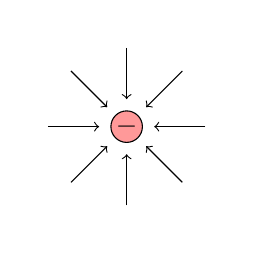
\begin{tikzpicture}
		\filldraw[white] (1.25, 1.25) rectangle (-1.25, -1.25);

		\coordinate (A1) at +(0:1);
		\coordinate (B1) at +(0:0.35);

		\coordinate (A2) at +(45:1);
		\coordinate (B2) at +(45:0.35);

		\coordinate (A3) at +(90:1);
		\coordinate (B3) at +(90:0.35);

		\coordinate (A4) at +(135:1);
		\coordinate (B4) at +(135:0.35);

		\coordinate (A5) at +(180:1);
		\coordinate (B5) at +(180:0.35);

		\coordinate (A6) at +(225:1);
		\coordinate (B6) at +(225:0.35);

		\coordinate (A7) at +(270:1);
		\coordinate (B7) at +(270:0.35);

		\coordinate (A8) at +(315:1);
		\coordinate (B8) at +(315:0.35);

		\draw[->] (A1) -- (B1);
		\draw[->] (A2) -- (B2);
		\draw[->] (A3) -- (B3);
		\draw[->] (A4) -- (B4);
		\draw[->] (A5) -- (B5);
		\draw[->] (A6) -- (B6);
		\draw[->] (A7) -- (B7);
		\draw[->] (A8) -- (B8);

		\filldraw[fill=red!40] (0, 0) circle (0.20);
		\draw (0, 0) node {$-$};
	\end{tikzpicture}
\end{figure}

\end{document}
\usepackage{amsmath}
